\section{Results}

Our experimental results are summarized in \tabref{tab:main_results}. We compare the baseline VGG-11 with standard ReLU activations against several variants of \methodname.

\begin{table}[h]
\centering
\caption{Main results on CIFAR-10 using VGG-11. We report Top-1 Test Accuracy and Expected Calibration Error (ECE). Best results in {\bf bold}.}
\label{tab:main_results}
\begin{tabular}{@{}lccc@{}}
\toprule
Method & Test Accuracy (\%) & ECE & Status \\
\midrule
{\bf ReLU Baseline} & {\bf 86.46} & 0.0236 & Success \\
\midrule
\textsc{SSA} (All Layers, Soft) & 10.21 & 0.0053 & Failed \\
\textsc{SSA} (All Layers, Hard) & 14.23 & 0.0041 & Failed \\
\midrule
{\bf \textsc{Mixed-SSA} (Last Layer, Soft)} & {\bf 83.09} & 0.0323 & Success \\
\textsc{Mixed-SSA} (Last Layer, Hard) & 10.38 & 0.0713 & Failed \\
\bottomrule
\end{tabular}
\end{table}

\para{Failure of Pure \textsc{SSA} Stacks}
A striking finding is the complete failure of networks where every activation is replaced by \methodname. Both "soft" and "hard" variants failed to exceed 15\% accuracy, which is only marginally better than random guessing. As shown in \figref{fig:accuracy}, these models show virtually no progress during the 10 epochs of training. We hypothesize that this is due to the "vanishing signal" problem: because the softmax outputs at each layer sum to 1.0, the average activation value is scaled down by a factor of $1/C$ at each layer. In a deep network like VGG-11, this attenuation becomes extreme, effectively zeroing out the signal and the gradients.

\para{Effectiveness of Hybrid Architectures}
In contrast, applying \methodname only at the final feature layer (\textsc{Mixed-SSA}) proved to be much more stable. The "soft" variant achieved 83.09\% accuracy, which is a respectable performance given the short training duration. This demonstrates that categorical sampling is a viable primitive when used as a specialized bottleneck rather than a general-purpose activation function. However, the "hard" variant of \textsc{Mixed-SSA} still failed to train, indicating that the high variance of discrete sampling gradients is particularly disruptive in competitive distributions.

\begin{figure}[h]
\centering
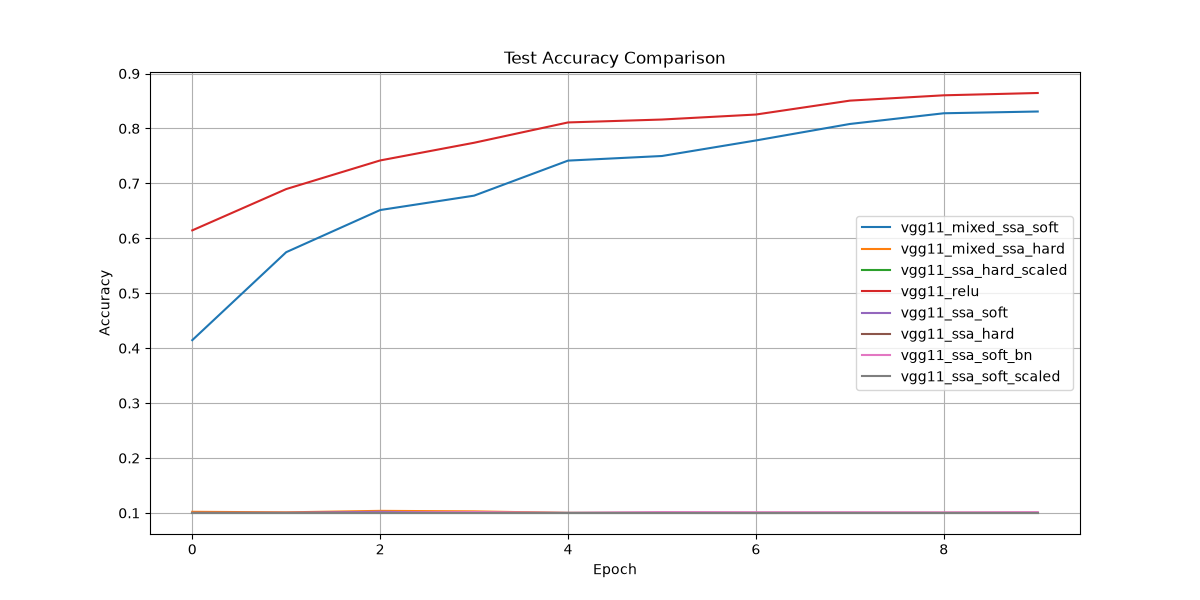
\includegraphics[width=0.7\linewidth]{figures/test_accuracy.png}
\caption{Test accuracy over 10 epochs of training on CIFAR-10. While the ReLU baseline and \textsc{Mixed-SSA} (Soft) converge, all variants using SSA at every layer or using "hard" sampling fail to show significant progress.}
\label{fig:accuracy}
\end{figure}

\para{Uncertainty Calibration}
We also measured the Expected Calibration Error (ECE) to see if the stochasticity of \methodname improves uncertainty quantification. Interestingly, \textsc{Mixed-SSA} (Soft) showed a slightly higher ECE (0.0323) than the ReLU baseline (0.0236). This suggests that while \methodname introduces stochasticity, it does not automatically lead to better-calibrated probabilities, at least without further tuning of the temperature parameter.
